Los rayos se dispersan en múltiples direcciones al incidir sobre una superficie rugosa o irregular. Esto forma imágenes que no son claras. La mayoría de los objetos en el ambiente reflejan la luz de forma difusa como la ropa, las paredes, el suelo, los árboles y otros.

\begin{figure}[H]
  \centering
  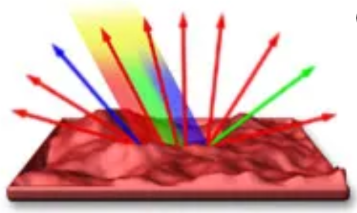
\includegraphics[scale=0.5]{imagenes/reflexion_difusa.png}
  \caption{Reflexión especular\cite{sncrflspcdif}}
\end{figure}
